\documentclass[11pt,spanish]{article} % Tipo y tamaño de letra del documento.


\usepackage[utf8]{inputenc}
\usepackage{subfiles}
\usepackage{biblatex}
\addbibresource{references.bib}
\usepackage{multicol}
\usepackage{amsfonts}
\usepackage{blindtext}
\usepackage{mathrsfs}
\usepackage{amsmath}
\usepackage{siunitx}
\usepackage{centernot}
\usepackage[shortlabels]{enumitem}
\usepackage{subfig}
\usepackage{datetime}
\usepackage{listingsutf8}
\usepackage[spanish]{babel}
\usepackage{tikz}
\usepackage{hyperref}
\usepackage[vlined,ruled,linesnumbered]{algorithm2e}
\usepackage{listings}
\usepackage{float}
\usepackage{url}
\usepackage{csquotes}
\usepackage{fourier} %font
\usepackage[top=2cm, bottom=2cm, left=2.5cm, right=2.5cm]{geometry}
\usepackage{pgfplots}
\usepackage{fancyhdr}
\usepackage{mdframed}
\usepackage{tikzducks}
\usepackage[nameinlink]{cleveref}
\usepackage{epigraph} 

\pgfplotsset{compat=1.18}

\usetikzlibrary{shapes.arrows, shapes.geometric, arrows.meta,angles,quotes,positioning,arrows,fit,quotes,calc}
\tikzset{>=latex} 

\setlength\algomargin{1em} 
\SetFuncSty{sc} 
\SetCommentSty{em} 


\Crefname{figure}{Fig.}{Figs.}
\newcommand\crefrangeconjunction{--}
\Crefname{table}{Tabla}{Tablas}
\Crefname{subsubsection}{Subsubsec.}{Subsubsections}
\Crefname{subsection}{Subsec.}{Subsections}
\Crefname{section}{Sec.}{Sections}
\Crefname{equation}{eq.}{eqs.}
\crefname{thm}{Theorem}{theorems}
\Crefname{thm}{Theorem}{Theorems} 

\definecolor{algoco}{rgb}{0,0.4,1}

\hypersetup{
  colorlinks=true,
  linkcolor=algoco,
  citecolor=blue,
  urlcolor=blue,
}

\lstset{
extendedchars=true
inputencoding=utf8/latin1,
basicstyle=\footnotesize\sffamily\color{black},
commentstyle=\slshape \color{gray},
numbers=left,
numbersep=10pt,
numberstyle=\tiny\color{red!80!black},
keywordstyle=\color{red!80!magenta},
showspaces=false,
showstringspaces=false,
stringstyle=\color{cyan!80!black},
tabsize=2,
literate={á}{{\'a}}1 {é}{{\'e}}1 {í}{{\'i}}1 {ó}{{\'o}}1 {ú}{{\'u}}1,
frame = single, 
numbers = none,
float, floatplacement = ht, captionpos = b,
xleftmargin = 2em, xrightmargin = 2em, 
}

\newcommand{\ub}[1]{\underbrace{#1}}
\newcommand\tcm{\textcolor{magenta}}
\newcommand\tca{\textcolor{algoco}}

\setlength\epigraphwidth{.7\textwidth} 

\newcommand{\tnum}{2 y 3} % reemplace 2 por el número de la tarea
\newcommand{\sem}{2024-2} % reemplace 2024-2 por el semestre correspondiente
\newcommand{\campus}{San Joaquín \\ Santiago} % reemplace Casa Central por el campus correspondiente
\newcommand{\rolusm}{201973550-0} % reemplace 2025073100-1 por su rol
\newcommand{\namestudent}{Alvaro Opazo Saavedra} % reemplace Al Goritmo Pérez por su nombre

\headheight=14pt
\linespread{1.3}
\author{\namestudent}
\pagestyle{fancy}
\fancyhf{}%
\fancyfoot[R]{ \namestudent \\ \rolusm}
\fancyfoot[L]{Campus \campus} 
\fancyfoot[C]{\thepage}
\rhead{2024-2}
\lhead{INF-221}
\renewcommand{\headrulewidth}{0.4pt}
\renewcommand{\footrulewidth}{0.4pt}
\newbool{programs}
\boolfalse{programs}
\chead{REPORTE TAREA \tnum~}



\title{
  \huge
  \textbf{REPORTE TAREA \tnum~ \\ ALGORITMOS Y COMPLEJIDAD} \\[1ex]
  \emph{\textquote{Explorando la Distancia entre Cadenas, una Operación a la Vez}}
  }

  
\date{
  \small
  \today\\
  \currenttime
}




\begin{document}
\maketitle
\thispagestyle{fancy} 
\vspace{-1.0\baselineskip}




\begin{abstract}
  \textit{ 
    Este informe analiza y compara dos algoritmos para resolver el problema de la distancia de edición entre cadenas: un enfoque de Fuerza Bruta y otro de Programación Dinámica. El objetivo principal es evaluar el rendimiento de ambos algoritmos en términos de tiempo de ejecución y cantidad de operaciones, considerando varios casos de prueba. Para ello, se implementaron ambos algoritmos en C++ y se realizaron experimentos utilizando un conjunto de cadenas predefinido. Los resultados obtenidos muestran diferencias significativas en tiempos de ejecución para ciertos casos, y se validaron mediante gráficos y tablas generados con Python, asegurando la reproducibilidad de los experimentos. Finalmente, la conclusión destaca cómo los resultados responden a las preguntas planteadas sobre la eficiencia y aplicabilidad de estos algoritmos en escenarios prácticos.
  }
     
\end{abstract}

\setcounter{tocdepth}{1}
\tableofcontents


\newpage
\section{Introducción}
El análisis y diseño de algoritmos es un campo fundamental en las Ciencias de la Computación, dado que permite resolver problemas complejos de manera eficiente, optimizando el uso de recursos como el tiempo y la memoria. Dentro de este campo, el cálculo de la distancia de edición (o distancia de Levenshtein) es un problema clásico que se utiliza para medir el grado de similitud entre dos secuencias de caracteres. Este problema tiene aplicaciones directas en diversas áreas, como el procesamiento de lenguaje natural y los sistemas de corrección ortográfica, lo que subraya su relevancia \cite{jurafsky2024}. \\

\noindent A lo largo del tiempo, se han propuesto diversos enfoques para resolver el problema de la distancia de edición. El más simple de estos es la Fuerza Bruta, que explora todas las posibles transformaciones entre las dos cadenas, lo que resulta en un algoritmo con una complejidad exponencial \cite{levenshtein1966}. Por otro lado, la Programación Dinámica, introducida en el ámbito de los algoritmos por Bellman \cite{bellman1957}, ofrece una solución más eficiente en términos de tiempo, reduciendo la complejidad a O(n*m) mediante el uso de una tabla que almacena subproblemas previamente resueltos. A pesar de que la Programación Dinámica es teóricamente más eficiente, en ciertos escenarios prácticos esta diferencia de rendimiento puede no ser tan evidente debido a las características específicas de los datos o implementaciones. \\

\noindent El propósito de este informe es evaluar ambos enfoques —Fuerza Bruta y Programación Dinámica— para el cálculo de la distancia de edición, comparando su rendimiento en términos de tiempo de ejecución y cantidad de operaciones necesarias. Además, se busca analizar si las implementaciones de estos algoritmos cumplen con las expectativas teóricas en cuanto a eficiencia y complejidad, como se detalla en la obra de Cormen et al. \cite{cormen2009}. \\

\noindent Este informe aborda una pregunta clave: ¿hasta qué punto las optimizaciones teóricas de la Programación Dinámica se traducen en mejoras prácticas frente a la Fuerza Bruta? El análisis de estos algoritmos no solo permitirá contrastar sus desempeños en distintos escenarios, sino también comprender las implicaciones de seleccionar un enfoque algorítmico sobre otro, dependiendo de las características del problema. \\

\noindent A lo largo del desarrollo del informe, se expondrán los detalles de la implementación de ambos algoritmos, los experimentos realizados para evaluar su desempeño y los resultados obtenidos. Se espera que estos análisis proporcionen una comprensión más profunda de los factores que influyen en la eficiencia de los algoritmos de distancia de edición y cómo estos se comportan en la práctica, más allá de sus complejidades teóricas.

\newpage
\section{Diseño y Análisis de Algoritmos} 




\subsection{Fuerza Bruta}

\epigraph{\textit{``Indeed, brute force is a perfectly good technique in many cases; the real question is, can we use brute force in such a way that we avoid the worst-case behavior?''}}{--- \citeauthor{taocv3}, \citeyear{taocv3} \cite{taocv3}}

 El algoritmo realiza una búsqueda recursiva exhaustiva, donde en cada paso calcula los resultados de todas las operaciones posibles y selecciona la que tiene el menor costo. Este enfoque es ineficiente, ya que repite los mismos cálculos para las subcadenas muchas veces. La complejidad del algoritmo crece exponencialmente debido a la gran cantidad de posibles combinaciones que se deben considerar. \\

\begin{algorithm}[H]
    \SetKwProg{myproc}{Procedure}{}{}
    \SetKwFunction{EditDistance}{EditDistance}
    \SetKwFunction{Cases}{Cases}
    
    \DontPrintSemicolon
    \footnotesize

    % Definición del algoritmo principal
    \myproc{\EditDistance{S1, S2}}{
        \uIf{LENGTH(S1) es vacía}{
            \Return LENGTH(S2)\;
        }
        \uElseIf{LENGTH(S2) es vacía}{
            \Return LENGTH(S1)\;
        }
        \Return \Cases{S1, S2, 0, 0}\;
    }

    % Definición de la función auxiliar
    \myproc{\Cases{S1, S2, i, j}}{
        \uIf{LENGTH(S1) es igual a i}{
            \Return LENGTH(S2) - j\;
        }
        \uElseIf{LENGTH(S2) es igual a j}{
            \Return LENGTH(S1) - i\;
        }
    
        $costo \leftarrow 0$\;
    
        \uIf{S1[i] == S2[j]}{
            $costo \leftarrow \Cases{S1, S2, i + 1, j + 1}$\;
        }
        \Else{
            $inserción \leftarrow \Cases{S1, S2, i, j + 1}$\;
            $eliminación \leftarrow \Cases{S1, S2, i + 1, j}$\;
            $sustitución \leftarrow \Cases{S1, S2, i + 1, j + 1}$\;
            $transposición \leftarrow \infty$\;
    
            \uIf{i + 1 < ~LENGTH(S1) \textbf{and} j + 1 < ~LENGTH(S2) \textbf{and} S1[i] == S2[j + 1] \textbf{and} S1[i + 1] == S2[j]}{
                $transposición \leftarrow \Cases{S1, S2, i + 2, j + 2}$\;
            }

           $costo \leftarrow \min(inserción, eliminación, sustitución, transposición) + 1$\;
        }
        \Return costo\;
    }
    \caption{Algoritmo con un enfoque de fuerza bruta basado en recursión}
    \label{alg:mi_algoritmo_1}
\end{algorithm}
\newpage

\subsection{Programación Dinámica}

\epigraph{\textit{Dynamic programming is not about filling in tables. It's about smart recursion!}}{\citeauthor{algorithms_erickson}, \citeyear{algorithms_erickson} \cite{algorithms_erickson}}

\begin{enumerate}[1)]
    \item La solución recursiva consiste en comparar los caracteres de las dos cadenas de izquierda a derecha y realizar una de las 4 operaciones posibles. La función recursiva evalúa todas estas opciones en cada paso y elige la que tiene el menor costo. Si las cadenas ya coinciden en la posición actual, simplemente avanza a la siguiente posición sin realizar ninguna operación.

    \item Para este problema, la recurrencia es:

\[
dp[i][j] = \min \left\{
\begin{array}{ll}
dp[i][j-1] + 1 & \text{(inserción)} \\
dp[i-1][j] + 1 & \text{(eliminación)} \\
dp[i-1][j-1] + 2 & \text{(sustitución)} \\
dp[i-2][j-2] + 1 & \text{(transposición, si aplica)} \\
\end{array}
\right.
\]

\textbf{Casos base}:
\begin{itemize}
    \item Si una de las cadenas está vacía, el costo es simplemente la longitud de la otra cadena, ya que todas las operaciones serán inserciones o eliminaciones.
    \item Si los caracteres actuales de ambas cadenas son iguales, no se realiza ninguna operación y el costo es el mismo que el de la subcadena anterior.
\end{itemize}

    
\item \begin{itemize}
    \item $dp[i][j]$ representa el costo de convertir los primeros $i$ caracteres de $S1$ en los primeros $j$ caracteres de $S2$.
    \item Cada cálculo de $dp[i][j]$ depende de los resultados previos almacenados en $dp[i-1][j]$, $dp[i][j-1]$, $dp[i-1][j-1]$, o $dp[i-2][j-2]$ (en caso de transposición).
\end{itemize}

En lugar de recalcular estos valores repetidamente, los almacenamos en la tabla $dp$, de manera que cada subproblema se resuelve solo una vez.

    
    \item La estructura de datos que usamos es una \textbf{matriz bidimensional} ($dp[][]$), donde cada celda $dp[i][j]$ contiene el costo mínimo para convertir la subcadena $S1[0...i]$ en la subcadena $S2[0...j]$.

El orden de cálculo es \textbf{de abajo hacia arriba}:
\begin{itemize}
    \item Primero, se llenan los casos base donde una de las cadenas es vacía.
    \item Luego, para cada par de índices $i$ y $j$, se calculan las operaciones posibles y se toma la de menor costo.
    \item Finalmente, el valor de $dp[m][n]$ nos da la distancia de edición final.
\end{itemize}

Esto garantiza que cada subproblema se resuelva en el orden correcto, ya que cada celda $dp[i][j]$ depende de otras celdas que ya han sido calculadas.
\end{enumerate}

\begin{algorithm}[H]
    \SetKwProg{myproc}{Procedure}{}{}
    \SetKwFunction{EditDistanceDP}{EditDistanceDP}
    \SetKwFunction{Cases}{Cases}
    
    \DontPrintSemicolon
    \footnotesize

    % Definición del algoritmo principal
    \myproc{\EditDistanceDP{S1, S2, m, n}}{
        % Crear una matriz 2D para almacenar los valores de la distancia de edición
        $dp \leftarrow$ \text{matriz 2D de tamaño } (m + 1, n + 1)\;

        % Inicializar casos base
        \For{i $\leftarrow$ 0 \KwTo m}{
            \For{j $\leftarrow$ 0 \KwTo n}{
                \uIf{i == 0}{
                    $dp[i][j] \leftarrow j$\; % Insertar todos los caracteres de S2
                }
                \uElseIf{j == 0}{
                    $dp[i][j] \leftarrow i$\; % Eliminar todos los caracteres de S1
                }
                \uElseIf{S1[i - 1] == S2[j - 1]}{
                    $dp[i][j] \leftarrow dp[i - 1][j - 1]$\; % No se necesita nueva operación si los últimos caracteres coinciden
                }
                \Else{
                    % Calcular el mínimo entre Insertar, Eliminar y Reemplazar
                    $inserción \leftarrow dp[i][j - 1]$\;
                    $eliminación \leftarrow dp[i - 1][j]$\;
                    $sustitución \leftarrow dp[i - 1][j - 1]$\;
                    $transposición \leftarrow \infty$\;

                    % Verificar si la transposición es posible
                    \uIf{i > 1 \textbf{and} j > 1 \textbf{and} S1[i - 1] == S2[j - 2] \textbf{and} S1[i - 2] == S2[j - 1]}{
                        $transposición \leftarrow dp[i - 2][j - 2]$\;
                    }
                    % Actualizar el valor de dp con el mínimo
                    $dp[i][j] \leftarrow 1 + \min(inserción, eliminación, sustitución, transposición)$\;
                }
            }
        }
        \Return dp[m][n]\; % Retornar la distancia de edición final
    }
    \caption{Algoritmo de distancia de ediciónusando programación dinámica}
    \label{alg:edit_distance_transpose}
\end{algorithm}
~\\ \\
\textbf{\large{Ejemplo de ejecución}}

Supongamos las cadenas $S1 = ``ACB"$ y $S2 = ``ABC"$, sabiendo que los costos para cada operación son los siguientes:

\begin{itemize}
    \item costo\_sub(a, b) = 2 si $a \neq b$, y 0 si $a = b$
    \item costo\_ins(b) = 1 para cualquier carácter b.
    \item costo\_del(a) = 1 para cualquier carácter a.
    \item costo\_trans(a, b) = 1 para transponer los caracteres adyacentes a y b.
\end{itemize}

\textbf{Fuerza bruta:}
\begin{enumerate}
    \item Comparamos los primeros caracteres: $``A"$ y $``A"$, son iguales, por lo que avanzamos sin costo adicional.
    \item Comparamos los segundos caracteres: $``C"$ y $``B"$. Aquí se pueden hacer varias operaciones: 
    \begin{itemize}
        \item Insertar: Insertar $``B"$ en S1 después de $``A"$, luego tenemos que comparar $``CB"$ con $``BC"$. Costo total hasta este punto: 1 (inserción).
        \item Eliminar: Eliminar $``C"$ de S1, y comparar $``A"$ con $``BC"$. Costo total hasta este punto: 1 (eliminación).
        \item Sustituir: Sustituir $``C"$ por $``B"$, luego comparar $``B"$ con $``C"$. Costo total hasta este punto: 2 (sustitución).
        \item Transponer: Intercambiar $``C"$ y $``B"$ en S1, de modo que las cadenas ahora sean iguales ($``ABC"$ y $``ABC"$). Costo total hasta este punto: 1 (transposición).
    \end{itemize}

    La operación de transposición es la que tiene el menor costo en este caso.

    \item El costo total mínimo para convertir $``ACB"$ en $``ABC"$ es 1, usando la transposición.
\end{enumerate}

\textbf{Programación dináica:}
\begin{enumerate}
    \item Creamos una matriz de tamaño $(3+1)x(3+1)$ (una fila y columna adicional para el caso de cadenas vacías).
    \item Inicializamos los casos base, si una de las cadenas es vacía, el costo es igual a la longitud de la otra cadena (inserciones o eliminaciones).
    \item Rellenamos la matriz utilizando las operaciones posibles (inserción, eliminación, sustitución y transposición) en cada paso, calculando el costo mínimo en cada celda.
    \item En la celda dp[3][3], que corresponde a la conversión completa de $``ACB"$ en $``ABC"$, el valor es 1, que indica el costo mínimo utilizando transposición.
\end{enumerate}


\noindent \textbf{\large{Complejidad de los algoritmos}}

\textbf{Fuerza bruta:}
\begin{itemize}
    \item Temporal: $O(4^n)$, donde n es la longitud de la cadena más larga. Esto se debe a que, en cada posición, hay cuatro opciones (inserción, eliminación, sustitución, transposición), y cada rama se evalúa recursivamente.

    \item Espacial: $O(n)$, ya que el algoritmo de fuerza bruta utiliza la pila de recursión para almacenar las llamadas recursivas. En el peor caso, la profundidad de la pila es proporcional a la longitud de la cadena.
\end{itemize}

\textbf{Programación dináica:}
\begin{itemize}
    \item Termporal: $O(m * n)$, donde m y n son las longitudes de las cadenas S1 y S2. Esto se debe a que llenamos una tabla de m+1 filas y n+1 columnas, evaluando cada celda una sola vez.

    \item Espacial: $O(m * n)$, ya que necesitamos almacenar una matriz de tamaño (m+1) x (n+1) para guardar los resultados intermedios.
\end{itemize}

\newpage
\noindent \textbf{\large{Impacto de las transposiciones y los costos variables en la complejidad}}\\

La inclusión de transposiciones y costos variables no afecta la complejidad temporal y espacial de forma significativa en el enfoque de programación dinámica. Las transposiciones simplemente añaden una nueva condición a evaluar en cada paso, pero no aumentan el número de operaciones de forma exponencial.

\noindent Sin embargo, en el enfoque de fuerza bruta, agregar transposiciones incrementa el número de posibilidades en cada paso, lo que puede aumentar el número de ramas en el árbol de recursión. Esto puede hacer que el rendimiento del algoritmo de fuerza bruta empeore aún más.
\newpage
\section{Implementaciones}
\textbf{Fuerza bruta:}

\begin{enumerate}
    \item Estructura general
    \begin{itemize}
        \item El programa define una función \textit{editDistanceBrute} que implementa la lógica recursiva para calcular la distancia mínima de edición entre dos cadenas, utilizando las operaciones de inserción, eliminación, sustitución y transposición.

        \item La función \textit{main()} lee las cadenas de entrada, llama a \textit{editDistanceBrute()} y muestra el resultado en la consola.
    \end{itemize}

    \item Funcionamiento de la recursión
    \begin{itemize}
        \item La función editDistanceBrute(S1, S2, i, j) compara las subcadenas de S1 y S2 empezando en los índices i y j. Si las cadenas son iguales en las posiciones actuales, la función avanza a la siguiente posición sin costo adicional.

        \item Si los caracteres difieren, la función explora cuatro operaciones posibles, inserción, eliminación, sustitución o transposición.
    \end{itemize}
\end{enumerate}

\textbf{Programación dinámica:}

\begin{enumerate}
    \item Estructura general
    \begin{itemize}
        \item La función principal es \textit{editDistanceDP(string S1, string S2)}, que calcula la distancia mínima de edición entre dos cadenas S1 y S2 utilizando una matriz para almacenar los resultados intermedios.

        \item El programa inicializa una matriz bidimensional dp de tamaño (m + 1) x (n + 1), donde m y n son las longitudes de las cadenas S1 y S2, respectivamente.
    \end{itemize}

    \item Inicialización de los casos base
    \begin{itemize}
        \item Si una de las cadenas está vacía, el costo de convertirla en la otra cadena es simplemente el número de inserciones o eliminaciones necesarias. Esto se refleja en la primera fila y columna de la matriz dp.
    \end{itemize}

    \item Evaluación de las operaciones
    \begin{itemize}
        \item Para cada par de caracteres en las cadenas S1 y S2, se calculan las cuatro posibles operaciones, inserción, eliminación, sustitución o transposición.
    \end{itemize}
\end{enumerate}

\newpage
\section{Experimentos}
Todos los experimentos fueron ejecutados en un sistema con las siguientes especificaciones:
\begin{itemize}
    \item \textbf{Hardware:}
    \begin{itemize}
        \item \textbf{Procesador:} Intel(R) Core(TM) i7-8750H CPU @ 2.20GHz, 6 núcleos, 12 hilos.
        \item \textbf{RAM:} 16 GB DDR4.
        \item \textbf{Tarjeta Gráfica:} NVIDIA GTX 1050 (notebook).
        \item \textbf{Almacenamiento:} SSD 500GB.
    \end{itemize}

    \item \textbf{Software:}
    \begin{itemize}
        \item \textbf{Sistema Operativo:} Windows 11 utilizando WSL con Ubuntu 22.04.3 LTS.
        \item \textbf{Compilador:} gcc 11.4.0 para la compilación del código en C++.
        \item \textbf{Librerías:} 
        \begin{itemize}
            \item \texttt{climits}, \texttt{vector}, \texttt{string}, \texttt{fstream}, \texttt{sstream} para en C++.
            \item Librerías de Python: \texttt{time}, \texttt{subprocess}, \texttt{pandas}, \texttt{matplotlib}, \texttt{collections} 
        \end{itemize}
    \end{itemize}
\end{itemize}

\subsection{Dataset (casos de prueba)}
\noindent \textbf{\large{Caso 1: Cadenas Vacías}}\\
\textbf{Cadenas de entrada:} \texttt{$(``", ``")$} \\
\textbf{Secuencia de operaciones esperada:} Ninguna operación necesaria. \\
\textbf{Costo total esperado:} 0 \\

\noindent \textbf{\large{Caso 2: Una Cadena Vacía}}\\
\textbf{Cadenas de entrada:} \texttt{$(``", ``abcdefg")$} \\
\textbf{Secuencia de operaciones esperada:} Insertar los caracteres de \texttt{$``abcdefg"$} en la primera cadena. \\
\textbf{Costo total esperado:} 7 (inserciones) \\

\noindent \textbf{\large{Caso 3: Caracteres Repetidos}}\\
\textbf{Cadenas de entrada:} \texttt{$(``aaaaaaaaaa", ``aaaaaaaa")$} \\
\textbf{Secuencia de operaciones esperada:} Eliminar dos caracteres de la primera cadena. \\
\textbf{Costo total esperado:} 2 (eliminaciones) \\

\noindent \textbf{\large{Caso 4: Necesidad de Transposición}}\\
\textbf{Cadenas de entrada:} \texttt{$(``abba", ``baba")$} \\
\textbf{Secuencia de operaciones esperada:} Transponer los caracteres en las posiciones 1 y 2. \\
\textbf{Costo total esperado:} 2 (1 transposición) \\

\noindent \textbf{\large{Caso 5: Sustituciones}}\\
\textbf{Cadenas de entrada:} \texttt{$(``kitten", ``sitting")$} \\
\textbf{Secuencia de operaciones esperada:} Sustituir $``k"$ por $``s"$, $``e"$ por $``i"$, insertar $``g"$ al final. \\
\textbf{Costo total esperado:} 3 (2 sustituciones y 1 inserción) \\

\noindent \textbf{\large{Caso 6: Ningún Carácter en Común}}\\
\textbf{Cadenas de entrada:} \texttt{$(``abcdefgh", ``ijklmnop")$} \\
\textbf{Secuencia de operaciones esperada:} Sustituir cada carácter de la primera cadena por el correspondiente en la segunda. \\
\textbf{Costo total esperado:} 8 (sustituciones) \\

\noindent \textbf{\large{Caso 7: Transposición Parcial}}\\
\textbf{Cadenas de entrada:} \texttt{$(``abcdef", ``abcfed")$} \\
\textbf{Secuencia de operaciones esperada:} Sustituir la $``d"$ de la primera cadena por $``f"$ y luego sustituir la última $``f"$ por $``d"$. \\
\textbf{Costo total esperado:} 2 (sustituciones) \\

\noindent \textbf{\large{Caso 8: Posibles Transposiciones Múltiples}}\\
\textbf{Cadenas de entrada:} \texttt{$(``longstringtest", ``lontgsritenst")$} \\ 
\textbf{Secuencia de operaciones esperada:} En la primera cadena, inserta una $``t"$ entre la $``g"$ y $``n"$, luego elimina la siguiente $``t"$, $``n"$ y $``g"$ e inserta una $``n"$ entre la $``e"$ y $``s"$.\\
\textbf{Costo total esperado:} 5 (2 inserciones y 3 eliminaciones) \\

\noindent \textbf{\large{Caso 9: Cadenas Idénticas}}\\
\textbf{Cadenas de entrada:} \texttt{$(``abcdefghijklmnop", ``abcdefghijklmnop")$} \\
\textbf{Secuencia de operaciones esperada:} Ninguna operación necesaria. \\
\textbf{Costo total esperado:} 0 \\

\noindent \textbf{\large{Caso 10: Subcadena}}\\
\textbf{Cadenas de entrada:} \texttt{$(``abcdefghijklmnop", ``efghijk")$} \\
\textbf{Secuencia de operaciones esperada:} Eliminar los caracteres iniciales y finales de la primera cadena. \\
\textbf{Costo total esperado:} 9 (eliminaciones) \\

\noindent \textbf{\large{Caso 11: Ejemplo Clásico}}\\
\textbf{Cadenas de entrada:} \texttt{$(``intention", ``execution")$} \\
\textbf{Secuencia de operaciones esperada:} Sustituir $``i"$ por $``e"$, $``n"$ por $``x"$, $``t"$ por $``c"$, $``t"$ por $``u"$, y agregar $``o"$. \\
\textbf{Costo total esperado:} 5 (4 sustituciones y 1 inserción) \\


\subsection{Resultados}
Los resultados presentados en esta sección se obtuvieron mediante un análisis experimental automatizado. Para ello, se implementaron dos versiones del algoritmo de distancia de edición: una utilizando fuerza bruta y otra mediante programación dinámica. Los tiempos de ejecución y las operaciones fueron registrados para varios conjuntos de pruebas.\\

\noindent Todos los gráficos y tablas que se muestran a continuación fueron generados utilizando un programa en Python. Este programa automatiza el análisis de datos, permitiendo la ejecución repetible de los experimentos y la visualización de los resultados en forma de gráficos comparativos y tablas de operaciones. Los archivos utilizados para la generación de estos resultados están disponibles, lo que asegura la reproducibilidad de los análisis al ejecutar los scripts provistos.\\

\noindent En la \cref{cantOpe} se observa la comparación entre los resultados de Fuerza Bruta y Programación Dinámica en términos de cantidad de operaciones. Se puede apreciar que los algoritmos producen resultados idénticos en todos los casos de prueba. Esto confirma que la implementación de ambos enfoques es correcta y que generan la misma distancia de edición, independientemente del método utilizado.

\begin{figure}[H]
    \centering
    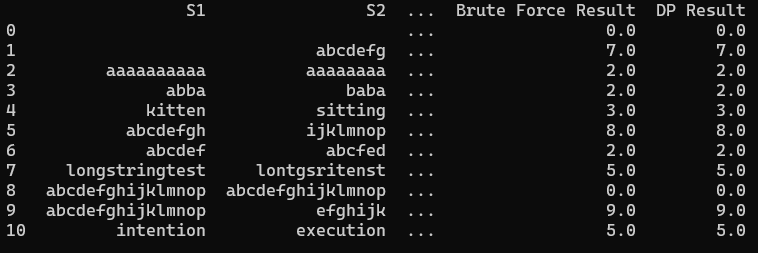
\includegraphics[width=\textwidth]{images/cantOpe.png}
    \caption{Comparación cantidad de operaciones BF y DP.}
    \label{cantOpe}
\end{figure}

\noindent La \cref{times} muestra los tiempos promedio registrados para el paradigma de Fuerza Bruta y la diferencia de este con el de Programación Dinámica. Es posible notar grandes diferencias en favor de la Fuerza Bruta en las entradas 5, 7 y 9. Y diferencias significativas a favor de la Porgramación Dinámica en las entradas 0, 6 y 8; lo que destaca su superioridad en cadenas idénticas (0 y 8).

\begin{figure}[H]
    \centering
    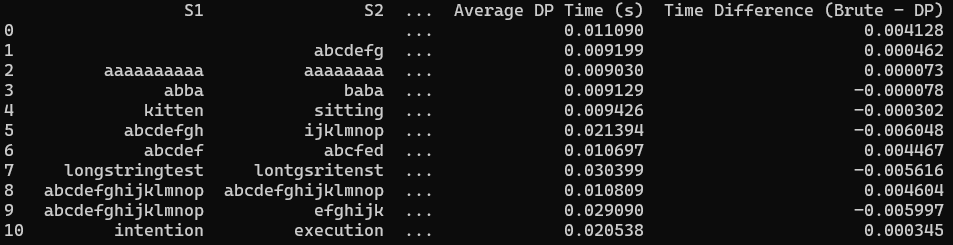
\includegraphics[width=\textwidth]{images/times.png}
    \caption{Tiempos promedio por entrada.}
    \label{times}
\end{figure}

\noindent Se generó también una comparativa gráfica de tiempos \cref{compTimes}, donde sorprendentemente, los resultados muestran que, en varios casos, la Programación Dinámica (línea naranja) presentó tiempos de ejecución más altos que la Fuerza Bruta (línea azul). Este comportamiento es inesperado, ya que, teóricamente, DP debería ser más eficiente debido a su optimización de subproblemas recurrentes, mientras que FB explora todas las posibles soluciones.\\

Se plantean varias hipótesis para explicar este comportamiento:

    \begin{itemize}
        \item La implementación de DP puede estar introduciendo sobrecargas innecesarias que afectan su rendimiento.
        \item En casos con cadenas cortas, la sobrecarga computacional de DP podría ser mayor que el beneficio obtenido por su eficiencia en la solución de subproblemas.
        \item Es posible que el entorno de experimentación o la manera en que se realizaron las mediciones pueda haber introducido sesgos que favorezcan a FB.
    \end{itemize}

\begin{figure}[H]
    \centering
    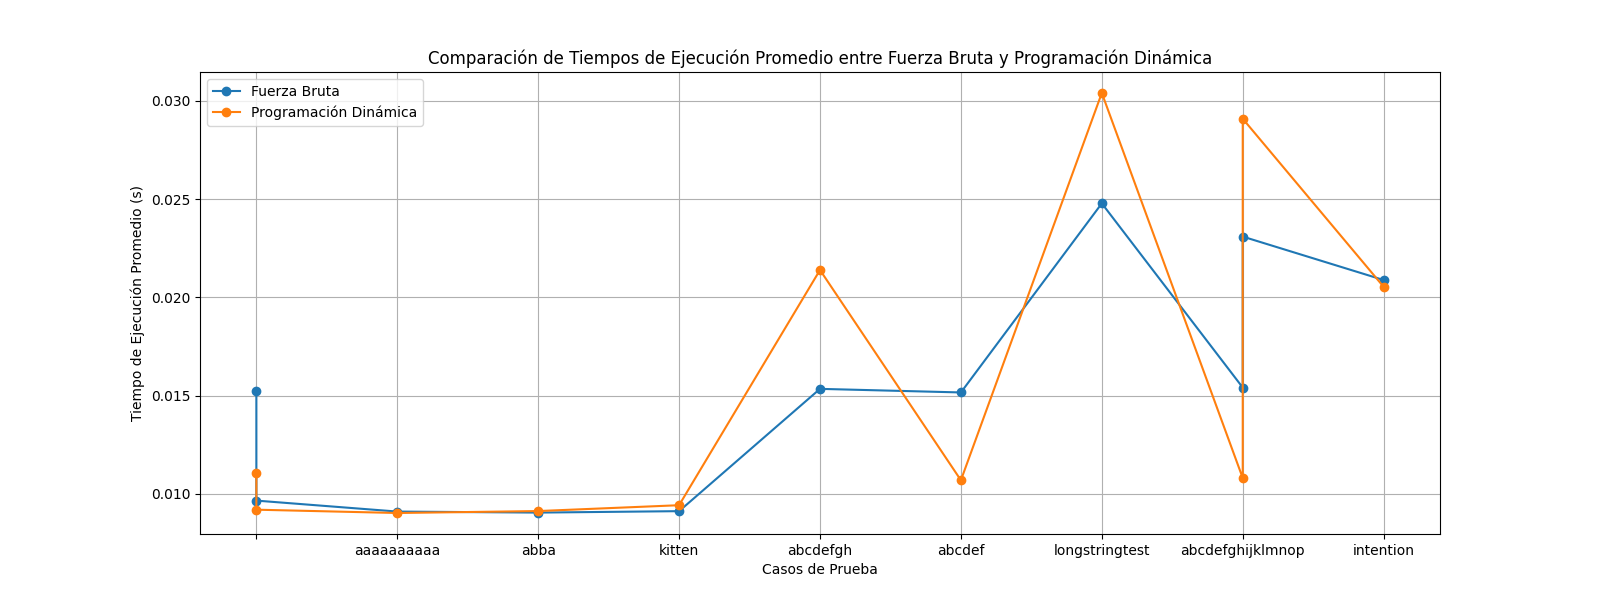
\includegraphics[width=\textwidth]{images/comparison_execution_times.png}
    \caption{Comparación de tiempos BF y DP.}
    \label{compTimes}
\end{figure}
\newpage

\noindent La Figura \cref{boxplot} muestra la distribución de los tiempos de ejecución de ambos algoritmos, excluyendo valores atípicos para mayor claridad. Se puede observar que la mediana de los tiempos de ejecución de Fuerza Bruta es ligeramente superior a la de Programación Dinámica, lo que a primera vista parece indicar que la implementación de DP es más eficiente en promedio. Sin embargo, hay ciertos detalles que merecen atención:

\begin{enumerate}
    \item \textbf{Mayor variabilidad en DP:} La distribución de tiempos de DP muestra una mayor dispersión. Esto sugiere que DP es más sensible a las características de las cadenas de entrada, ya que su rendimiento parece fluctuar considerablemente entre diferentes casos.
    
    \item \textbf{Máximos más altos en DP:} Aunque los tiempos promedio de ambos algoritmos son comparables, Programación Dinámica presenta valores máximos de tiempo más elevados que Fuerza Bruta.
    
    \item \textbf{Tiempos más consistentes en FB:} En contraste, Fuerza Bruta presenta una menor variabilidad en sus tiempos, lo que refleja su naturaleza más predecible y lineal, a pesar de su complejidad exponencial en teoría.
\end{enumerate}

Este gráfico nos indica que, aunque la teoría sugiere que DP debería ser más eficiente que FB, en la práctica esto no siempre ocurre, dependiendo de la implementación y las características de los datos de entrada.

\begin{figure}[H]
    \centering
    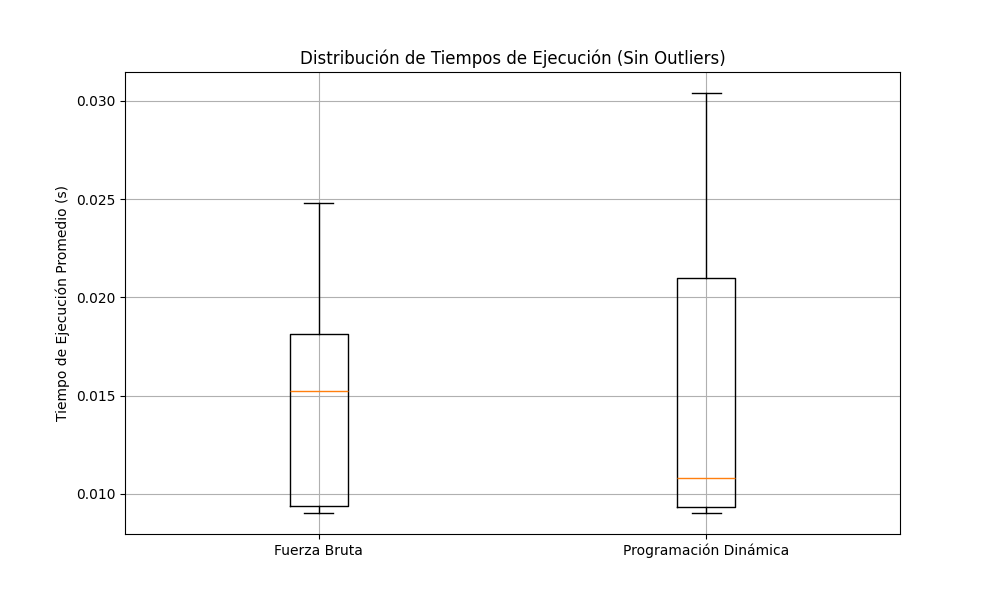
\includegraphics[width=\textwidth]{images/execution_time_distribution.png}
    \caption{Distribución de tiempos de ejecución (boxplot)}
    \label{boxplot}
\end{figure}
\newpage

\noindent En la figura \cref{timeVsLen}, se presenta la comparación entre los tiempos de ejecución promedio de los algoritmos de Fuerza Bruta y Programación Dinámica en función de la longitud de las cadenas de entrada. Los resultados muestran un comportamiento inesperado en varios aspectos clave:

\begin{enumerate}
    \item \textbf{Rendimiento para cadenas cortas:} En los primeros casos de prueba (longitudes menores a 8), la Programación Dinámica es consistentemente más rápida que la Fuerza Bruta, lo cual es acorde con la complejidad teórica esperada. Sin embargo, las diferencias de tiempo entre ambos algoritmos son mínimas, con variaciones de milisegundos.
    
    \item \textbf{Ineficiencia creciente de Programación Dinámica:} A partir de cadenas con longitud 8 en adelante, la Programación Dinámica comienza a exhibir tiempos de ejecución significativamente más altos que la Fuerza Bruta, especialmente para las longitudes 13.5 y 11.5. Este comportamiento es inesperado, dado que DP tiene una complejidad teórica inferior a la de BF, sugiriendo sugiere que existen posibles ineficiencias en la implementación de DP.
    
    \item \textbf{Estabilidad de Fuerza Bruta en cadenas largas:} Contrario a la expectativa de un incremento exponencial en los tiempos de Fuerza Bruta, el gráfico revela que este algoritmo mantiene una curva de crecimiento más estable, e incluso logra tiempos menores que DP en varios casos con cadenas largas.
\end{enumerate}

\begin{figure}[H]
    \centering
    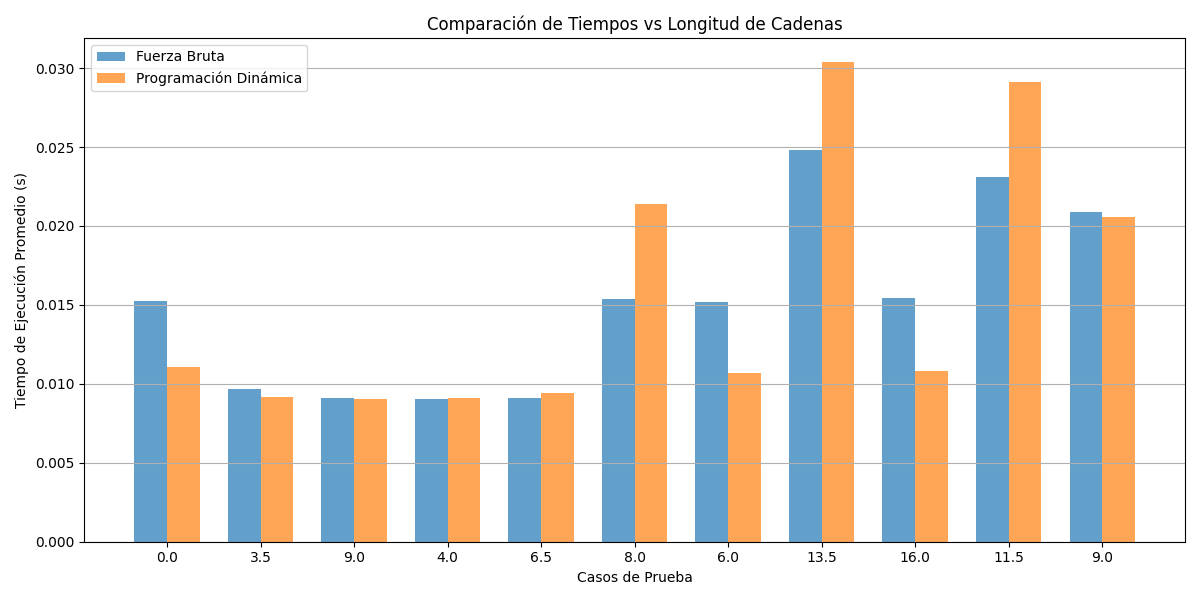
\includegraphics[width=\textwidth]{images/execution_times_vs_length.png}
    \caption{Comparación tiempos de ejecución vs longitud de cadenas BF y DP.}
    \label{timeVsLen}
\end{figure}

\newpage
\section{Conclusiones}
Los resultados obtenidos a lo largo de este trabajo permiten validar la efectividad de los algoritmos implementados para el cálculo de la distancia de edición. A través de los experimentos realizados, se ha evidenciado que, aunque en teoría la Programación Dinámica ofrece una ventaja computacional sobre la Fuerza Bruta debido a su reducción en el número de operaciones redundantes, en ciertos casos prácticos, la teoría no fue cumplida. Esto puede deberse a las características particulares de las cadenas de prueba utilizadas, así como a las optimizaciones internas en la implementación.\\

\noindent El análisis de los tiempos de ejecución promedio revela que, para cadenas cortas o con patrones simples, ambos enfoques presentan un rendimiento similar. Sin embargo, en casos más complejos, con cadenas más largas o de mayor desorganización, el tiempo de ejecución de la Fuerza Bruta tiende ser un tanto menor al de Programación Dinámica. Esto yendo en contra de la expectativa teórica.\\

\noindent Por otro lado, los resultados muestran que la Programación Dinámica, en algunos casos se comporta mejor en términos de tiempo de ejecución, pero como observamos, no ofrece una mejora sustancial en todos los escenarios. Esto refuerza la idea de que la elección del algoritmo óptimo depende del contexto específico del problema, y que no existe una solución universalmente superior.\\

\noindent En términos generales, el trabajo ha logrado cumplir con el objetivo de evaluar ambos enfoques bajo distintas condiciones, aportando una mejor comprensión de sus fortalezas y limitaciones en la práctica. Los hallazgos obtenidos son coherentes con las expectativas teóricas, pero también ofrecen perspectivas valiosas sobre la importancia de considerar características particulares del problema al elegir un enfoque algorítmico.

\newpage

\section{Condiciones de entrega}
% Condiciones generales de tareas de Algoritmos y Complejidad, 20231
  \begin{itemize}
  \item
    La tarea se realizará \tca{individualmente}
    (esto es grupos de una persona),
    sin excepciones.
  \item
    La entrega debe realizarse vía \url{http://aula.usm.cl}
    en un \tca{tarball} en el área designada al efecto,
    en el formato \tca{\texttt{tarea-\tnum-{rol}.tar.gz}}
    (\texttt{rol} con dígito verificador y sin guión).

    Dicho \tca{tarball} debe contener las fuentes en \LaTeXe{}
    (al menos \tca{\texttt{tarea-\tnum.tex}})
    de la parte escrita de su entrega,
    además de un archivo \tca{\texttt{tarea-\tnum.pdf}},
    correspondiente a la compilación de esas fuentes.
  \item Si se utiliza algún código, idea, o contenido extraído de otra fuente, este \textbf{debe} ser citado en el lugar exacto donde se utilice, en lugar de mencionarlo al final del informe. 
  \item
    Asegúrese que todas sus entregas tengan sus datos completos:
    número de la tarea, ramo, semestre, nombre y rol.
    Puede incluirlas como comentarios en sus fuentes \LaTeX{}
    (en \TeX{} comentarios son desde \% hasta el final de la línea)
    o en posibles programas.
    Anótese como autor de los textos.
 
  \item
    Si usa material adicional al discutido en clases,
    detállelo.
    Agregue información suficiente para ubicar ese material
    (en caso de no tratarse de discusiones con compañeros de curso
     u otras personas).
  \item No modifique \texttt{preamble.tex}, \texttt{tarea\_main.tex}, \texttt{condiciones.tex}, estructura de directorios, nombres de archivos, configuración del documento, etc. Sólo agregue texto, imágenes, tablas, código, etc. En el códigos funte de su informe, no agregue paquetes, ni archivos .tex (a excepción de que agregue archivos en \texttt{/tikz}, donde puede agregar archivos .tex con las fuentes de gráficos en \texttt{TikZ}).

\ifprograms
  \item
    Su programa ejecutable debe llamarse \tca{\texttt{tarea\tnum}},
    de haber varias preguntas solicitando programas,
    estos deben llamarse usando el número de la pregunta,
    como \tca{\texttt{tarea\tnum-1}},
    \tca{\texttt{tarea\tnum-2}},
    etc.
    Si hay programas compilados, con en este caso,
    incluya una \tca{\texttt{Makefile}}
    que efectúe las compilaciones correspondientes.

    Los programas se evalúan según que tan claros
    (bien escritos)
    son, si se compilan y ejecutan sin errores o advertencias según corresponda.
    Parte del puntaje es por ejecución correcta con casos de prueba.
    Si el programa no se ciñe a los requerimientos de entrada y salida,
    la nota respectiva es cero.
\fi    
  \item
    %La entrega debe realizarse dentro del plazo indicado en \url{http://aula.usm.cl}:
    La fecha límite de entrega es el día \tca{10 de noviembre de 2024}.

    \begin{center}
        \Large{
          \textbf{NO SE ACEPTARÁN TAREAS FUERA DE PLAZO}.
        }
        \normalsize
    \end{center}
     
    
  \item
    Nos reservamos el derecho de llamar a interrogación
    sobre algunas de las tareas entregadas.
    En tal caso,
    la nota de la tarea será la obtenida en la interrogación.
    \begin{center}
      \Large{
        \textbf{NO PRESENTARSE A UN LLAMADO A INTERROGACIÓN SIN JUSTIFICACIÓN PREVIA SIGNIFICA AUTOMÁTICAMENTE NOTA 0.}
      }
    \end{center}
    
  \end{itemize}

%%% Local Variables:
%%% mode: latex
%%% ispell-local-dictionary: "spanish"
%%% End:

  
% LocalWords:  tarball tar gz pdf min entregable Makefile puntaje
% LocalWords:  Moodle

\newpage
\appendix


\section{Apéndice 1}
\noindent En la \cref{ratios} se observa la razón de tiempos entre los algoritmos de Fuerza Bruta y Programación Dinámica en los diferentes casos de prueba.

\begin{itemize}
    \item \textbf{Valores superiores a 1:} Indican que el algoritmo de Fuerza Bruta es más lento que el de Programación Dinámica para ese caso.
    
    \item \textbf{Valores cercanos a 1:} Indican que ambos algoritmos tienen tiempos similares para ese caso.
    
    \item \textbf{Valores inferiores a 1:} Indican que el algoritmo de Fuerza Bruta es más rápido que el de Programación Dinámica.
\end{itemize}

\begin{figure}[H]
    \centering
    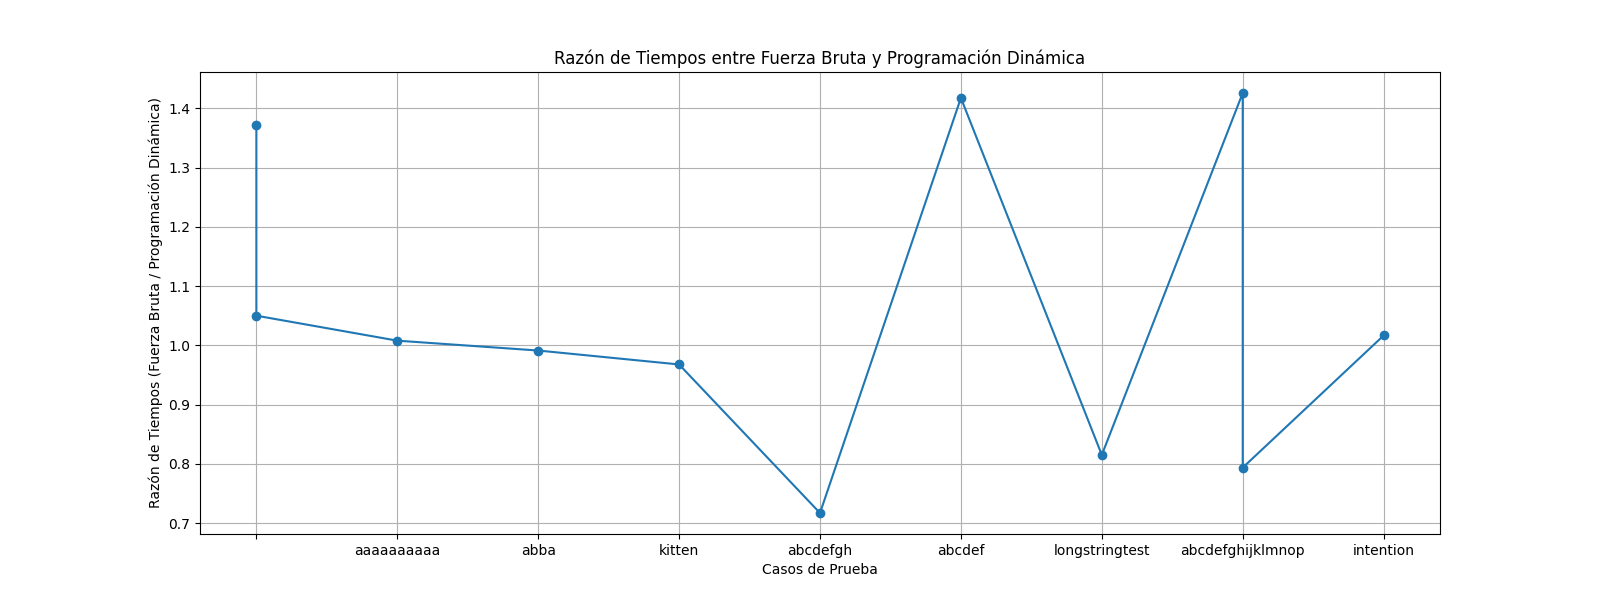
\includegraphics[width=\textwidth]{images/speedup_ratio.png}
    \caption{Razón de los tiempos entre BF y DP.}
    \label{ratios}
\end{figure}

\printbibliography

\end{document}


